\documentclass[a4paper,english,11pt]{scrartcl}
\usepackage{mystyle}
%opening\usepackage{subfig}
\hyphenation{ana-lysis Page-Rank intuitively}
\title{Link-based algorithms}
\subtitle{Text Based Information Retrieval (H02C8A)}
\author{Li Quan}
\date{April 28, 2011}
\renewcommand{\vec}[1]{\mathbf{#1}}

\begin{document}
\maketitle
%, i.e., solving the eigensystem $A\pi=\pi$, where $A$ is the link matrix of the web, using the (iterative) power method. 

\tableofcontents

\clearpage
\section{Introduction}
In this paper, we investigate the link analysis algorithm PageRank~\cite{pap,Page1998}. Various aspects of this algorithm have already been studied extensively (e.g.,~\cite{function,Bryan,fiddling,deeper,Langville:2006:GPB:1146372}). This paper answers the following questions:
\begin{enumerate}
 \item What is the distribution of PageRank values as the number of iterations approaches infinity? We consider the convergence properties of the power iteration to solve the eigenvector problem with respect to the need of the damping factor.
 \item What is the trade-off for the damping factor? In particular, the influence on the convergence rate and variability of PageRank values is explained.
 \item What are methods to personalise the PageRank values? We also discuss their advantages and disadvantages.
\end{enumerate}

\begin{notation}
Matrices and vectors are denoted upright boldface and scalars italic. 
Vectors are assumed to be column vectors.
E.g., $\vec{A}$ is a matrix, $\vec{v}$ a vector, and $\alpha$ a scalar.
Unless stated explicitely otherwise, symbol names are used as in~\cite{ams}. The PageRank vector is denoted by $\boldsymbol{\pi}^T$.
\end{notation}

\section{Calculating PageRank}
% \begin{quote}} 
% 
% \end{quote}

\subsection{Using no damping factor}
We calculate the PageRank vector for the graph of \emph{sample-tiny.txt}, visualised in~\autoref{fig:graph1}. First we use the basic power iteration with no damping factor, where we completely preserve the hyperlink matrix $\vec{H}$.

\begin{figure}[hbpt]\footnotesize
 \begin{center}
 
\begin{tikzpicture}[>=latex,line join=bevel,]
%%
\node (1) at (63bp,28bp) [draw,ellipse] {1};
  \node (0) at (9bp,46bp) [draw,ellipse] {0};
  \node (3) at (171bp,28bp) [draw,ellipse] {3};
  \node (2) at (117bp,65bp) [draw,ellipse] {2};
  \node (4) at (225bp,9bp) [draw,ellipse] {4};
  \draw [->] (2) ..controls (132.41bp,54.443bp) and (145.07bp,45.766bp)  .. (3);
  \draw [->] (0) ..controls (34.824bp,50.543bp) and (74.746bp,57.566bp)  .. (2);
  \draw [->] (1) ..controls (89.329bp,28bp) and (128.7bp,28bp)  .. (3);
  \draw [->] (1) ..controls (88.402bp,22.03bp) and (128.1bp,13.328bp)  .. (162bp,10bp) .. controls (176.84bp,8.5434bp) and (193.73bp,8.3543bp)  .. (4);
  \draw [->] (3) ..controls (186.85bp,22.423bp) and (197.88bp,18.541bp)  .. (4);
  \draw [->] (0) ..controls (24.851bp,40.716bp) and (35.885bp,37.038bp)  .. (1);
  \draw [->] (1) ..controls (78.407bp,38.557bp) and (91.072bp,47.234bp)  .. (2);

%
\end{tikzpicture}

\end{center}
\caption{The web graph of \emph{sample-tiny.txt}.\label{fig:graph1}}
\end{figure}

\autoref{tab:simple1} shows the PageRank values after each iteration: after 4~iterations, the result is the null vector. This result is obviously meaningless. Node~4 drains all the importance from the web, in each iterative step taking some of the importance of nodes~1 and 3, but not passing it on to other nodes, as it has no outgoing links---it is a so-called dangling node~\cite{ams}.


\begin{table}[hbpt]
  \centering\footnotesize
 \begin{tabular}{c c S S S S S}
  \toprule
      && \multicolumn{5}{c}{PageRank value of node} \\\cmidrule(l){3-7}
{$k$} && \multicolumn{1}{c}{0} & \multicolumn{1}{c}{1}  & \multicolumn{1}{c}{2}  & \multicolumn{1}{c}{3}  & \multicolumn{1}{c}{4}  \\ \midrule
0     && 0.2000 & 0.2000 & 0.2000 & 0.2000 & 0.2000 \\
1     && 0.0000 & 0.1000 & 0.1667 & 0.2667 & 0.2667 \\
2     && 0.0000 & 0.0000 & 0.0333 & 0.2000 & 0.3000 \\
3     && 0.0000 & 0.0000 & 0.0000 & 0.0000 & 0.3000 \\
4     && 0.0000 & 0.0000 & 0.0000 & 0.0000 & 0.0000 \\
\vdots&& \multicolumn{1}{c}{\vdots} & \multicolumn{1}{c}{\vdots} & \multicolumn{1}{c}{\vdots} & \multicolumn{1}{c}{\vdots} & \multicolumn{1}{c}{\vdots}\\
  \bottomrule
 \end{tabular}
  \caption{Distribution of $\boldsymbol{\pi}^T$ of the graph \emph{sample-tiny.txt} in the $k$th iteration.\label{tab:simple1}}
\end{table}

\subsubsection*{Dangling nodes}
Dangling nodes are certainly not an exception in real-world graphs: for some subsets of the web, dangling nodes make up 80 percent of the collection's page~\cite{deeper}.
Various methods to deal with these nodes have therefore been proposed~\cite{Lee03afast,dangling,deeper,math}.

A standard approach is to modify $\vec{H}$ as follows: $\vec{S}=\vec{H}+\vec{A}$, where $\vec{A}=\vec{d}\vec{w}^T$. The vector $\vec{d}$ identifies dangling nodes ($d_i$ is $1$ if the $i$th row-sum of $\vec{H}$ is 0, and 0 otherwise) and $\vec{w}$ is a probability distribution vector~\cite{math}. 
An obvious choice for $\vec{w}$ is the use of an uniform probability distribution: this is equivalent to adding artifical links from dangling nodes to all pages. 

When the power iteration is now applied to the same example, the algorithm converges (for $\epsilon=\num{1e-4}$, after about 15 iterations) to the stationary vector \[\boldsymbol{\pi}^T=(0.0769, 0.1154, 0.1539, 0.2692, 0.3846).\]


% 
% \autoref{tab:simple2} shows the distribution of the PageRank values of the pages as the number of iterations approaches infinity.
% 
% \begin{table}[hbpt]
%   \centering\footnotesize
%  \begin{tabular}{c c S S S S S}
%   \toprule
%       && \multicolumn{5}{c}{PageRank value of node} \\\cmidrule(l){3-7}
% {$i$} && \multicolumn{1}{c}{0} & \multicolumn{1}{c}{1}  & \multicolumn{1}{c}{2}  & \multicolumn{1}{c}{3}  & \multicolumn{1}{c}{4}  \\ \midrule
% 0     && 0.2000 & 0.2000 & 0.2000 & 0.2000 & 0.2000 \\
% 1     && 0.0400 & 0.1400 & 0.2067 & 0.3067 & 0.3067 \\
% 2     && 0.0613 & 0.0813 & 0.1280 & 0.3147 & 0.4147 \\
% 3     && 0.0829 & 0.1136 & 0.1407 & 0.2380 & 0.4247 \\
% 4     && 0.0849 & 0.1264 & 0.1643 & 0.2634 & 0.3609 \\
% 5     && 0.0722 & 0.1146 & 0.1568 & 0.2786 & 0.3778 \\
% \vdots&& \multicolumn{1}{c}{\vdots} & \multicolumn{1}{c}{\vdots} & \multicolumn{1}{c}{\vdots} & \multicolumn{1}{c}{\vdots} & \multicolumn{1}{c}{\vdots} \\
% % 6     && 0.0756 & 0.1117 & 0.1499 & 0.2706 & 0.3924 \\
% % 7     && 0.0785 & 0.1163 & 0.1535 & 0.2656 & 0.3862 \\
% % 8     && 0.0772 & 0.1165 & 0.1552 & 0.2695 & 0.3816 \\
% % 9     && 0.0763 & 0.1149 & 0.1538 & 0.2704 & 0.3846 \\
% 10    && 0.0769 & 0.1151 & 0.1534 & 0.2690 & 0.3856 \\
% \vdots&& \multicolumn{1}{c}{\vdots} & \multicolumn{1}{c}{\vdots} & \multicolumn{1}{c}{\vdots} & \multicolumn{1}{c}{\vdots} & \multicolumn{1}{c}{\vdots} \\
% 15    && 0.0769 & 0.1154 & 0.1539 & 0.2692 & 0.3846 \\
% %\vdots&& \multicolumn{1}{c}{\vdots & \vdots & \vdots & \vdots & \vdots \\
%   \bottomrule
%  \end{tabular}
%   \caption{Distribution of PageRank values of the nodes of the graph \emph{sample-tiny.txt} in the $i$th iteration.\label{tab:simple2}}
% \end{table}

\subsection{Using a damping factor}
The matrix $\vec{S}$ is stochastic, it can be proven that stochastic matrices always have stationary vectors \cite{stationary}. 
However, in general, we also have to use a damping factor $\alpha$ to \emph{ensure convergence of the power iteration algorithm to an unique stationary probability vector, i.e., the PageRank, which has all strictly positive values} (proven by the Perron–Frobenius theorem)~\cite{ams,Langville:2006:GPB:1146372,math}.

\subsubsection*{The need for the damping factor}
Consider for instance the web graphs shown in \autoref{fig:graph100}, for which our current version of the power iteration fails. 

The graph in Figure~\ref{figa} has a subdominant eigenvalue $|\lambda_2|=1$ and fails to converge. 
A necessary condition for the convergence of the power iteration is that it is applied on a matrix that has subdominant eigenvalues with magnitude smaller than the dominant eigenvalue  (i.e., $|\lambda_i|<|\lambda_1|=1, \textrm{ for }i =2\ldots n$). To satisfy the condition, the matrix $\vec{S}$ has to be \emph{primitive}~\cite{ams}.

\begin{figure}[Hbpt]
\centering
 \subfloat[Cyclic graph]{\label{figa}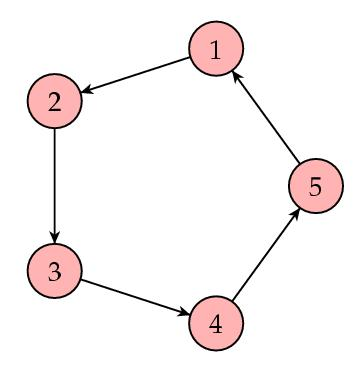
\includegraphics[width=0.3\textwidth]{cyclic}}
\subfloat[Non strongly connected graph]{\label{figb}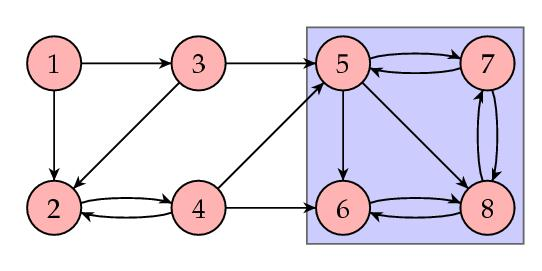
\includegraphics[width=0.5\textwidth]{reduciblewithbox}}
\caption{Calculating PageRanks without a damping factor fails for certain graphs. (Examples are taken from~\cite{ams}.)}
\label{fig:graph100}
\end{figure}

For the graph in Figure~\ref{figb}, another problem arises. The power iteration converges to $\boldsymbol{\pi}^T=(0,0,0,0,0.12,0.24,0.24,0.4)$. Clearly, nodes~1--4 should have some importance (there are nodes that link to them), but the importance sink (drawn in blue) drains the importance of these nodes in a way similar to dangling nodes as discussed above~\cite{ams}.
In general, we want $\boldsymbol{\pi}^T$ to have all strictly positive entries; a way of forcing this is making $\vec{S}$ \emph{irreducible} which is equivalent to considering only strongly connected graphs~\cite{fiddling,Langville:2006:GPB:1146372}.

\subsubsection*{The Google matrix}
To summarize, we have to modify $\vec{S}$ using the damping factor $\alpha$ in such a way that it is both primitive and irreducible~\cite{ams}.
This damping factor models the random surfer, who, with probability $\alpha$, follows a link of the current page, and with probability $1 − \alpha$ teleports to a random page using any other means (e.g., a bookmark).

This finally results in the \emph{Google matrix}:
\begin{align}
\vec{G} &=\alpha \vec{S} + (1-\alpha)\vec{E} =  \alpha \vec{H} + \alpha \vec{A} + (1-\alpha)\vec{E}
                   \label{eq:google}                                                                                                                    
\end{align}
with the teleportation matrix $\vec{E}= \vec{e}\vec{v}^T$, where $\vec{e}$ is the vector of ones and $\vec{v}$ a probability distribution vector called the teleportation vector. A straight-forward choice---which we will use for the moment---is again the uniform distribution $\vec{v}= \frac{1}{n}\vec{e}$.


\section{Damping factor trade-offs}
\subsection{Damping factor value}
The damping factor $\alpha$ represents a weighting of the matrices $\vec{S}$ and $\vec{E}$ in the Google matrix.
As $\alpha\rightarrow{}0$, the web has a link between any two pages and we lose the original hyperlink structure of the web.
On the other spectrum, as $\alpha\rightarrow{}1$, the random surfer only uses the hyperlink structure: this has the consequence that important pages (i.e., pages that happen to be linked by many other pages, or by few important ones) will be visited more often by the random surfer and therefore will have higher PageRank scores~\cite{ams}. 

Clearly, we want important pages to have higher PageRank scores; however, when we take a large value of $\alpha$, the convergence of the power method will be very slow (it is easily proven that the convergence of the power iteration depends on the rate at which $\alpha^k\rightarrow0$~\cite{function,Langville:2006:GPB:1146372}). 

Contrary to some popular belief, $\alpha\approx1$ does \emph{not} deliver ``better'' PageRank values~\cite{function}. Intuitively, this is easily explained: users do not surf on the web by just clicking on hyperlinks all the time.
Additionally, sensitivity issues ($
 |\frac{d\pi_i(\alpha)}{d\alpha} | \leq \frac{1}{1-\alpha}
$) can arise when the damping factor is chosen close to 1 \cite{function,Langville:2006:GPB:1146372}.

\begin{figure}[Hhbpt] \centering
 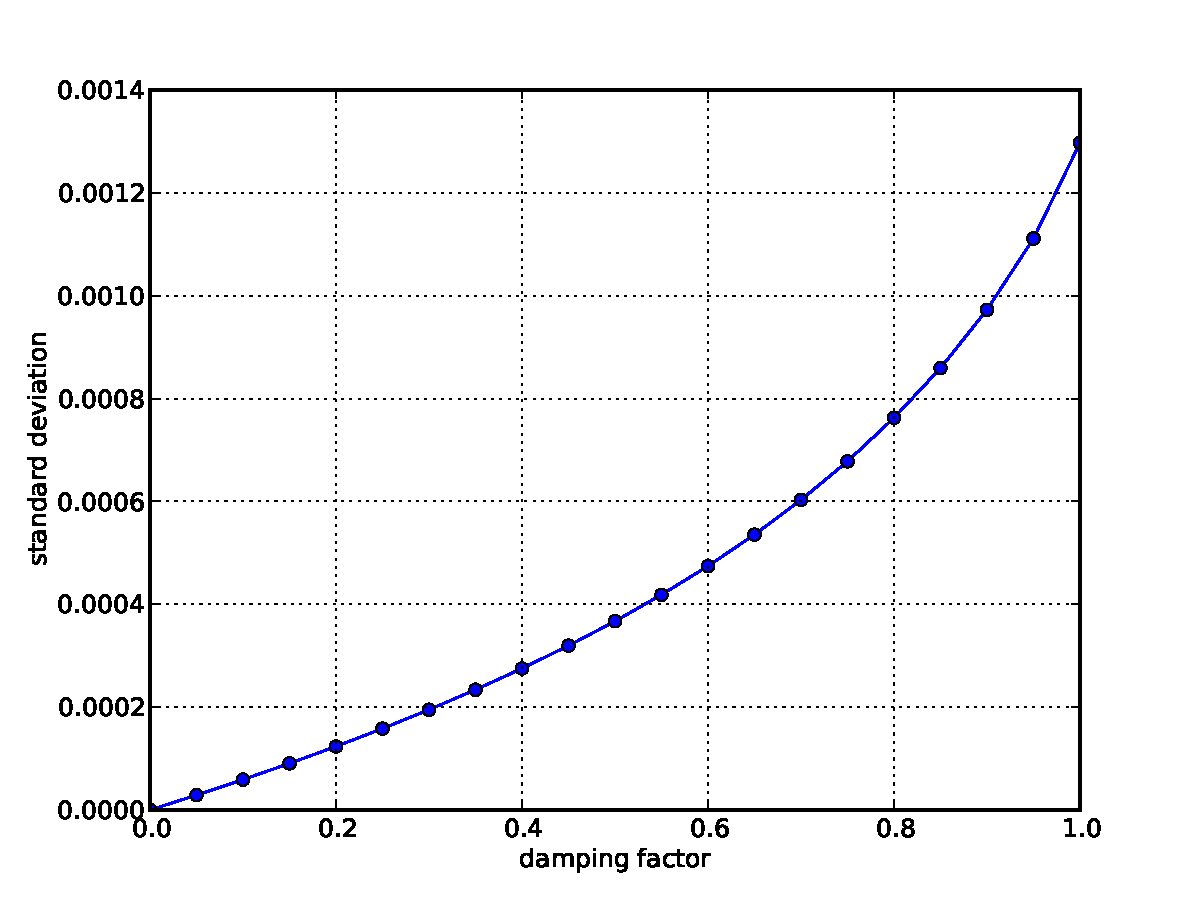
\includegraphics[width=0.75\textwidth]{standard_deviation}
 \caption{Damping value and standard deviation of PageRank scores. \label{fig:std}}

 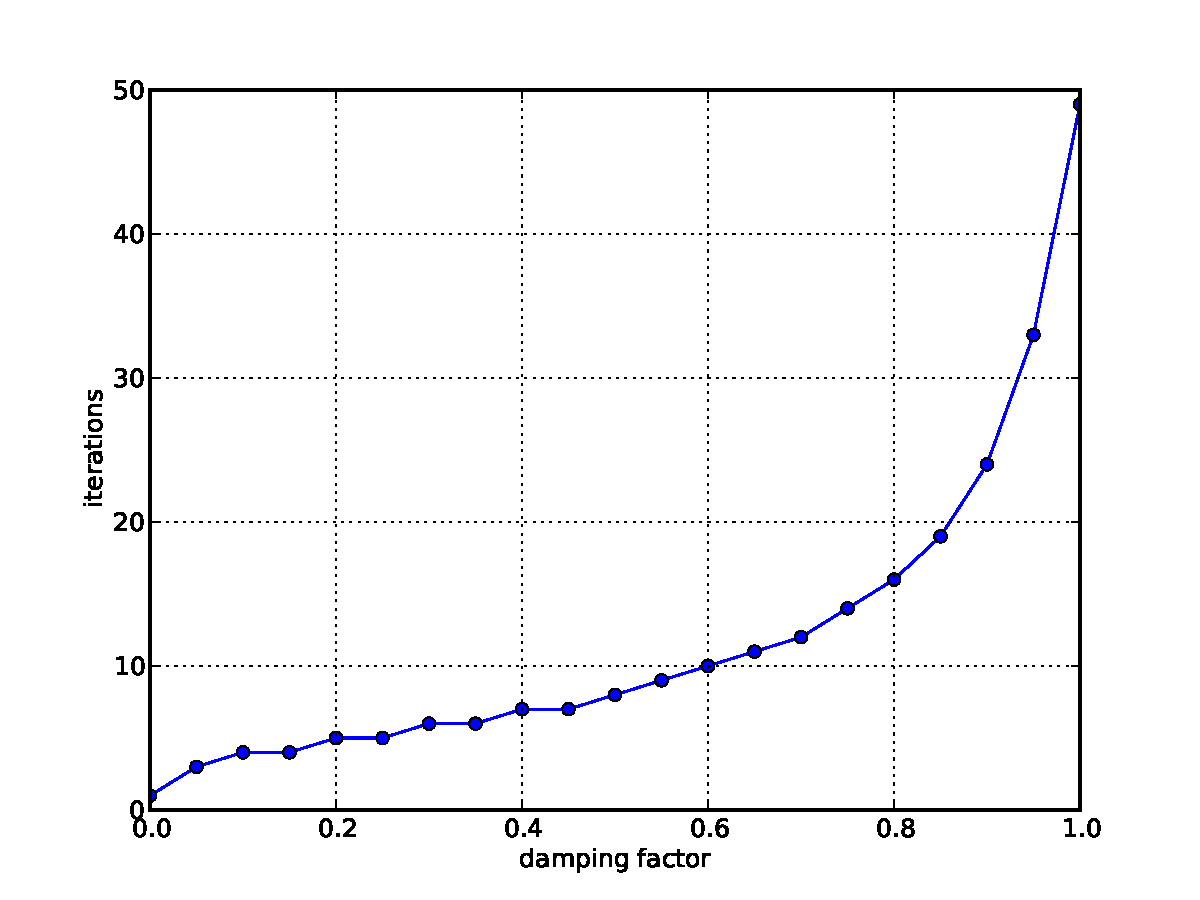
\includegraphics[width=0.75\textwidth]{iterations}
 \caption{Damping value and number of iterations required for convergence of PageRank scores ($\epsilon=\num{1e-4}$). \label{fig:iterations}}
\end{figure}

\subsection{Experiments}
To illustrate these trade-offs, we calculate the PageRank values of the web graph given in \emph{sample-large2.txt}, with various damping values from $0$ to $1$ in increments of $0.05$. 

\autoref{fig:std} shows the standard deviation of the PageRank values and \autoref{fig:iterations} the number of iterations for convergence. 
As expected, for small values of $\alpha$, the algorithm takes less iterations to converge and the standard deviation is smaller, compared to larger values of $\alpha$.
% 
% Now recall that most of the entries in $\vec{H}$ are zero; on average, only ten entries per column are nonzero. Therefore, evaluating HI k requires only ten nonzero terms for each entry in the resulting vector. Also, the rows of A are all identical as are the rows of 1. Therefore, evaluating AI k and 1I k amounts to adding the current importance rankings of the dangling nodes or of all web pages. This only needs to be done once. 

\section{Personalisation of PageRank}
\label{sec:personalisation}

Personalised search is a hot area since some predict them
as the future~(e.g.,~\cite{personalizations, Matthijs:2011:PWS:1935826.1935840,Stamou:2009:SPT:1499116.1499120,Wedig:2006:LAQ:1150402.1150497}). The papers \cite{personalizations} and \cite{deeper} give a good overview on this subject in the context of PageRank. 

The teleportation vector $\vec{v}$ in the Google matrix (Eq.~\ref{eq:google}) is also known as the \emph{personalisation vector}~\cite{math}. As its name suggests, this vector can be adjusted to model the random surfer's tendencies by introducing a bias on the probabilities that certain pages are chosen. 

While the concept of full personalisation sounds wonderful in theory, doing this in practice is still computationally infeasible~\cite{deeper}. The personalisation currently used by Google\footnote{See~\url{http://www.google.com/psearch}.} is based on the user's web history and location. This restricts the way personalisation is done (users can't have direct influence on how their results are personalised)~\cite{thesis}, but allows for reasonable efficient computations while allowing some degree of personalisation. 

Nevertheless, the concept of the personalisation vector is useful and has also been used for other purposes such as
controlling spamming done by link farms~\cite{deeper,math}.
We now discuss some proposed methods to personalise PageRank more in-depth.

\subsection{Topic-Sensitive PageRank}
First consider a more restricted version of full personalisation called Topic-Sensitive PageRank~\cite{personalizations}. The basic idea is to precompute a set of importances for a page with respect to various topics (by setting the personalisation vector values higher corresponding to pages relevant to those topics)~\cite{ilprints750}. (Note that the damping factor $\alpha$ has a direct influence on the amount of biasing \cite{personalizations}.)

At query-time, the PageRank value is weighted according to this set of importances. There should be enough topics to have a useful model; using too many topics will however have a negative impact on the efficiency~\cite{personalizations,ilprints750}. This approach is suitable for query-sensitive PageRanking, but does not allow for ``true'' user personalisation.
% 
% \begin{figure}[hbpt] \centering
%  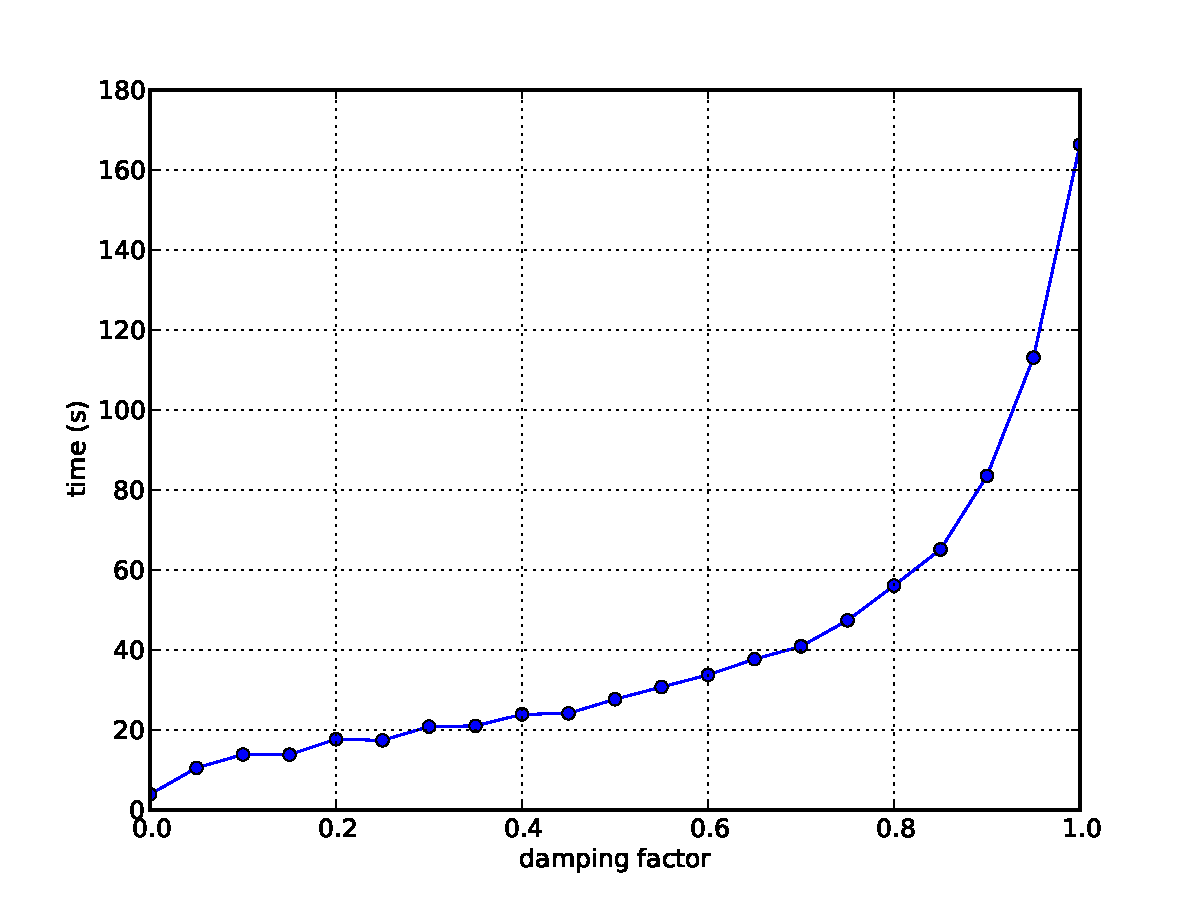
\includegraphics[width=0.75\textwidth]{times}
%  \caption{Damping value and computation time required for convergence of PageRank scores ($\epsilon=\num{1e-4}$). \label{fig:times}}
% \end{figure}thesis

\subsection{Real-time personalisation}
%Two promising approaches on real-time personalised search engines \cite{deeper} are discussed. 

In \cite{Jeh:2003:SPW:775152.775191} a linear relationship between personalisation vectors and their corresponding personalised PageRank vectors is identified. This relationship allows the personalised PageRank vector to be expressed as a linear combination of vectors that are called basis vectors~\cite{deeper}. (The number of basis vectors is a parameter in the algorithm.) 

The computation of the basis vectors is done by a scalable dynamic
programming approach. At query time, an \emph{approximation} to the personalised PageRank
vector is constructed from the precomputed basis vectors~\cite{ilprints750,Jeh:2003:SPW:775152.775191,deeper}.

\paragraph{}
Another possible approach involves the BlockRank algorithm~\cite{Kamvar03exploitingthe}. It was originally designed as
a method for accelerating the computation of the standard PageRank vector by finding a good starting
vector, but has also been suggested as a method to create personalised PageRank vectors~\cite{deeper}. 

BlockRank is an aggregation method that lumps sections of the web by hosts, using the natural structure of the web. 
BlockRank consists of three main steps~\cite{deeper}:
\begin{enumerate}
 \item First, local PageRanks for pages in a host are computed independently using the link structure of the host.
 \item In the next step, these local PageRanks are weighted by the importance of the corresponding
host. 
\item Finally, the usual PageRank algorithm is run using the weighted aggregate of the local
PageRank vectors as the starting vector. By assuming a web surfer can only teleport to hosts (rather
than individual pages), personalisation can be accounted for in the second step. 
\end{enumerate}
This algorithm gives the personalised PageRank vector, \emph{not} an approximation in contrast to the previous approach,
with relatively low overhead~\cite{deeper}. 
%\clearpage

\section{Conclusion}
The damping factor is crucial for the workings of the PageRank algorithm, in particular for the convergence of the power iteration. The damping factor allows an intuitive model of a random surfer, who not only surfs on the web by clicking links, but can also teleport to some page (with probability $1-\alpha$). 

An important question remains the value of $\alpha$: from empirical experiments (and supposedly used by Google), $\alpha=0.85$, seems a good trade-off between convergence rate and ``true'' page rankings~\cite{Page1998,math}. However, no analytical justifications have been given; some researchers have also advocated the use of $\alpha=0.5$ \cite{Avrachenkov06asingular,function,Bressan:2009:CDC:1506844.1506853}.

Personalisation makes the once query-independent, user-independent PageRanking calculations query-dependent, user-dependent and more calculation-laden~\cite{deeper}.
While significant research has been done to minimise the effort associated with personalised results, search engines are still far from producing real-time fully personalised results~\cite{thesis}. 


\clearpage
\bibliographystyle{acm}
\bibliography{biblio}
% \nocite{*}
\end{document}
